
%*******************************************************************************
%***********************************    Background   *****************************
%*******************************************************************************
%!TEX root = 0.main.tex

\setcounter{page}{1}



%********************************** %First Section  **************************************
\section {Introduction and general background} 

\subsection{Introduction}

[Intro to neural networks]\\
Neural Networks are popular algorithms for regression and classification tasks. In complex problems where we don't know the important features of the input data, neural networks can automatically "learn" these features through multiple combinations of linear and non-linear transformations of the input [Better explain this]. This characteristic makes them the optimal tool for complex tasks such as image classification, image segmentation, speech recognition and natural language processing.\\

[Intro to CNN]\\
Convolutional Neural Networks (CNNs) are a specific class of neural networks whose connectivity structure has been specifically designed for image recognition and segmentation. For this purpose, they have been designed to be equivariant to translation of the input. This means that if used in an image classification task, a translation of the input image will not result in a change of class. Thanks to their design, training of CNNs is faster - thanks to the smaller number of parameters to be learned compared to a fully connected NN- easier -since there's no need of artificially augmenting the dataset with translated copies of the same image: the network does not need to learn translation invariance, it was designed to be translation equivariant at the start- and leads to very accurate results.\\

[Intro to Spherical CNN]\\
Spherical CNNs are a variation of CNNs that have been designed to deal with spherical data, whose design make them equivariant to rotations of the input.  Examples of tasks where data is naturally represented on a sphere are (i) climate science, where data is sampled on the surface of the Earth, (ii) cosmology, where observations are naturally projected on a sphere centered around the observer (see Figure \ref{fig:cosmicradiation}), and (iii) in virtual reality, where the images are represented on a sphere centered around the player. Being able to come up with designs that are 	equivariant to rotations brings to these tasks all the advantages that traditional CNNs have brought for traditional (euclidean) image classification tasks. \textbf{[Talk about convolutions on the sphere]}

\begin{figure}
	\label{fig:cosmicradiation}
	\centering
	\caption{Cosmic microwave background map, the oldest electromagnetic radiation in the universe. Source: Wikipedia}
	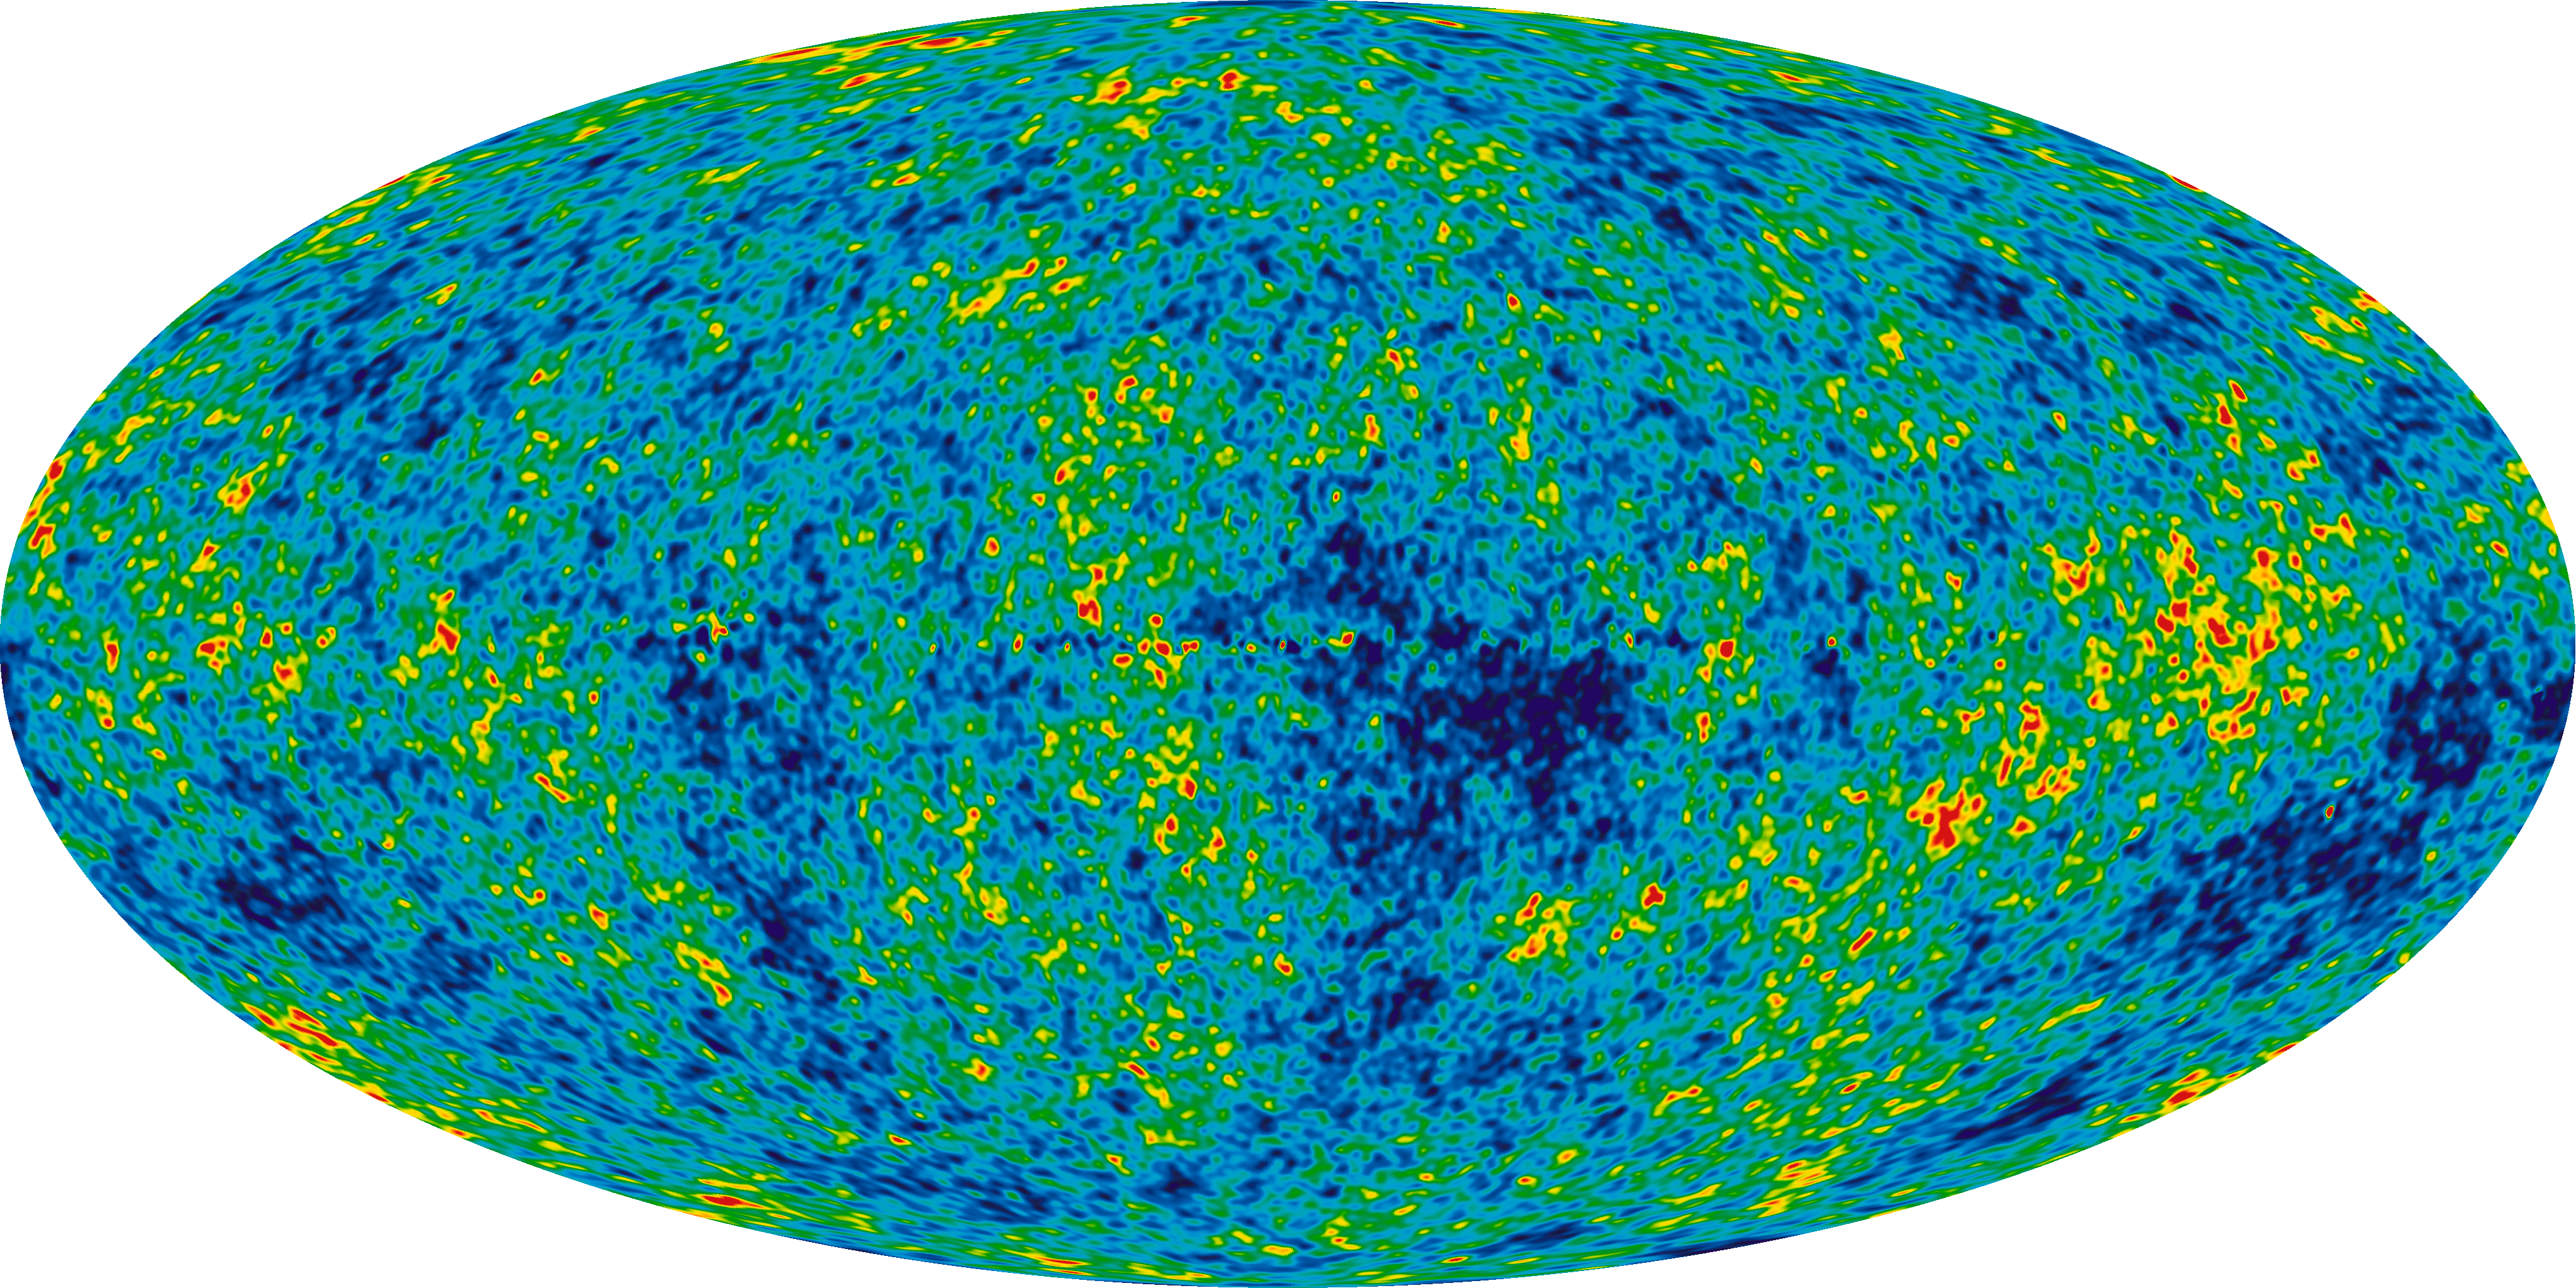
\includegraphics[width=0.4\textwidth]{figs/literaturereview/WMAP.png}
\end{figure}

[Intro to Graph CNN and DeepSphere]\\
One of the main issues with Spherical Neural Networks is the computational complexity of the learning phase. Deferrard et al \cite{DeepSphere} proposed an architecture that is almost equivariant to rotations, but limit the computational complexity of the algorithm to be linear with the dimension of the input data. The idea is to construct a suitable graph whose vertices represent the pixels of the image, think about the pixel values as a function on the vertices of this graph and then use graph convolutions to approximate the spherical convolution. Through the graph convolution we can indeed avoid the expensive computation of the spherical Fourier transform.
\subsection{Fourier Transforms and Convolutions on the 2-Sphere}


\subsection{Spherical Convolutional Neural Networks}

\subsection{Graph Spectral Theory}

\subsection{Deep Sphere V1.0}

\subsection{Belkin's trinity}
